\documentclass[a4paper,12pt]{letter}

\usepackage{amsmath}
\usepackage{amssymb}
\usepackage{nopageno}
\usepackage{amsmath}
%\usepackage{enumitem}
% \usepackage{mathtools}
%\usepackage{eqnarray,amsmath}
\usepackage[a4paper, total={7.5in, 11.25in}]{geometry}
%\usepackage[margin=2.5cm]{geometry}
\usepackage[utf8]{inputenc}
\usepackage[T1]{fontenc}
\usepackage{lmodern}
%\usepackage{amsmath, amssymb}
\usepackage{setspace}
\setstretch{1.2}
\usepackage{pgfplots}
\pgfplotsset{compat=1.18}


\begin{document}

\begin{center}
 (KTXFI1EBNF) Physics I.  Supplementary Matterial\\ \smallskip
March~8,~2026
 \end{center}

\begin{enumerate}

\item \textit{Find the launch angle that maximizes the range of a projectile for a given initial speed $v$.}

\medskip
  
The horizontal range $R$ of a projectile is given by the formula:
\begin{equation}
    R(\theta) = \frac{v^2 \sin(2\theta)}{g}
\end{equation}
where:
\begin{itemize}
    \item $v$ is the initial launch speed,
    \item $\theta$ is the launch angle,
    \item $g$ is the acceleration due to gravity.
\end{itemize}

To find the maximum range, we differentiate $R$ with respect to $\theta$ and set the derivative to zero:
\begin{equation}
    \frac{dR}{d\theta} = \frac{v^2}{g} \cdot \frac{d}{d\theta}(\sin(2\theta)) = \frac{2v^2 \cos(2\theta)}{g} = 0
\end{equation}

For this expression to be zero, we must have:
\begin{equation}
    \cos(2\theta) = 0 \implies 2\theta = 90^\circ \implies \theta = 45^\circ
\end{equation}

The following plot compares trajectories at different angles. The $45^\circ$ curve reaches the furthest distance.

\begin{center}
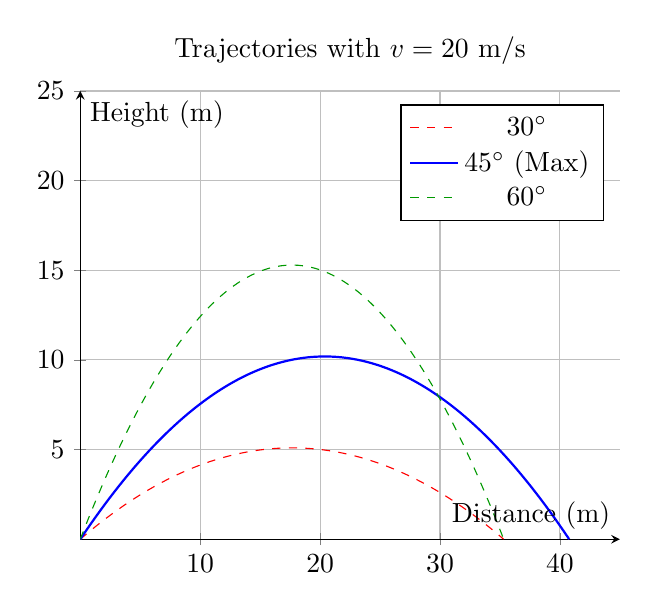
\begin{tikzpicture}
\begin{axis}[
    axis lines = middle,
    xlabel = {Distance (m)},
    ylabel = {Height (m)},
    xmin=0, xmax=45,
    ymin=0, ymax=25,
    grid = major,
    legend pos = north east,
    title = {Trajectories with $v = 20$ m/s}
]
% Trajectory formula: y = x*tan(theta) - (g*x^2)/(2*v^2*cos(theta)^2)
% g=9.81, v=20

% 30 degrees
\addplot [domain=0:35.3, samples=100, color=red, dashed] 
{x*tan(30) - (9.81*x^2)/(2*20^2*cos(30)^2)};
\addlegendentry{$30^\circ$}

% 45 degrees (Maximum)
\addplot [domain=0:40.77, samples=100, color=blue, thick] 
{x*tan(45) - (9.81*x^2)/(2*20^2*cos(45)^2)};
\addlegendentry{$45^\circ$ (Max)}

% 60 degrees
\addplot [domain=0:35.3, samples=100, color=green!60!black, dashed] 
{x*tan(60) - (9.81*x^2)/(2*20^2*cos(60)^2)};
\addlegendentry{$60^\circ$}

\end{axis}
\end{tikzpicture}
\end{center}

The maximum range is achieved at a launch angle of \textbf{45 degrees}. At this angle, the range formula becomes $R_{max} = \frac{v^2}{g}$.

% -------------------------------------------------------------------------------------------------

\item \textit{Calculate the impact distance of a projectile given an initial speed $v=1500\,km/s$ and an angle $\alpha=75^{\circ}$. At what other angle is the range identical?}

\medskip
  
Calculate the impact distance (range) of a projectile given:
\begin{itemize}
    \item Initial speed: $v = 1500\,\text{m/s} = 1.5 \times 10^3\,\text{m/s}$
    \item Launch angle: $\alpha = 75^\circ$
\end{itemize}
Find the other angle that yields the same range.

The horizontal range $R$ is given by:
\begin{equation}
    R = \frac{v^2 \sin(2\alpha)}{g}
\end{equation}

Substituting the given values ($g \approx 9.81\,\text{m/s}^2$):
\begin{align*}
    R &= \frac{(1.5 \times 10^3)^2 \cdot \sin(2 \cdot 75^\circ)}{9.81} \\
    R &= \frac{2.25 \times 10^{6} \cdot \sin(150^\circ)}{9.81} \\
    R &= \frac{2.25 \times 10^{6} \cdot 0.5}{9.81} \approx 1.146 \times 10^{5}\,\text{m}
\end{align*}

The range is identical for the complementary angle:
\begin{equation}
    \alpha' = 90^\circ - \alpha = 90^\circ - 75^\circ = 15^\circ
\end{equation}

The plot below illustrates the paths for both $75^\circ$ and $15^\circ$ (scaled for visualization).

\begin{center}
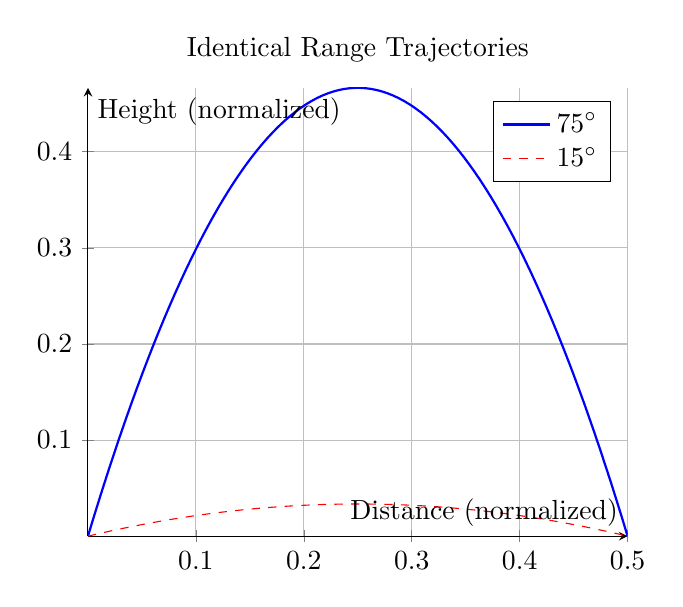
\begin{tikzpicture}
\begin{axis}[
    axis lines = middle,
    xlabel = {Distance (normalized)},
    ylabel = {Height (normalized)},
    grid = major,
    legend pos = north east,
    title = {Identical Range Trajectories}
]
% Using normalized units for plotting purposes
\addplot [domain=0:0.5, samples=100, color=blue, thick] {x*tan(75) - (0.5*x^2)/(cos(75)^2)};
\addlegendentry{$75^\circ$}

\addplot [domain=0:0.5, samples=100, color=red, dashed] {x*tan(15) - (0.5*x^2)/(cos(15)^2)};
\addlegendentry{$15^\circ$}
\end{axis}
\end{tikzpicture}
\end{center}

The impact distance is approximately $1.146 \times 10^{5}$ meters. The range is also identical at a launch angle of $15^\circ$.

% -------------------------------------------------------------------------------------------------

\item \textit{A projectile is launched at an angle of $60^\circ$ with an initial velocity of $25\,\text{m/s}$.}
Calculate:
\begin{enumerate}
    \item[(a)] The time to reach the peak of the trajectory.
    \item[(b)] The maximum height.
    \item[(c)] The horizontal range (impact distance).
    \item[(d)] The total time of flight.
\end{enumerate}

\medskip

Given values: $v_0 = 25\,\text{m/s}$, $\alpha = 60^\circ$, and $g = 9.81\,\text{m/s}^2$.

\begin{enumerate}

\item[(a)] Time to peak: The vertical velocity component is $v_y = v_0 \sin\alpha - gt$. At the peak, $v_y = 0$:
\begin{equation}
    t_{peak} = \frac{v_0 \sin\alpha}{g} = \frac{25 \cdot \sin(60^\circ)}{9.81} \approx 2.21\,\text{s}
\end{equation}

\item[(b)] Maximum height
\begin{equation}
    H = \frac{v_0^2 \sin^2\alpha}{2g} = \frac{25^2 \cdot (0.866)^2}{19.62} \approx 23.90\,\text{m}
\end{equation}

\item[(c)] Horizontal range
\begin{equation}
    R = \frac{v_0^2 \sin(2\alpha)}{g} = \frac{25^2 \cdot \sin(120^\circ)}{9.81} \approx 55.18\,\text{m}
\end{equation}

\item[(d)] Total time of flight. Since the launch and impact heights are the same:
\begin{equation}
    t_{total} = 2 \cdot t_{peak} \approx 4.42\,\text{s}
\end{equation}
\end{enumerate}

\begin{center}
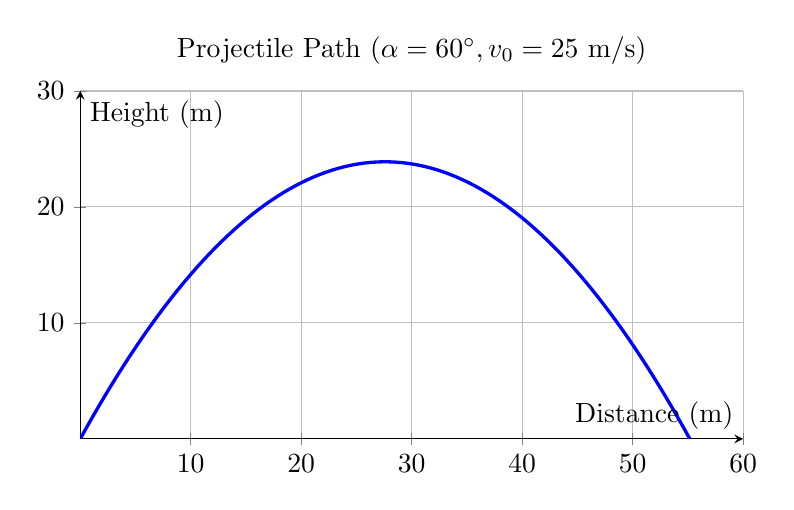
\begin{tikzpicture}
\begin{axis}[
    axis lines = middle,
    xlabel = {Distance (m)},
    ylabel = {Height (m)},
    xmin=0, xmax=60,
    ymin=0, ymax=30,
    grid = major,
    width=10cm, height=6cm,
    title={Projectile Path ($\alpha=60^\circ, v_0=25$ m/s)}
]
\addplot [
    domain=0:55.18, 
    samples=100, 
    color=blue,
    very thick,
]
{x*tan(60) - (9.81*x^2)/(2*25^2*cos(60)^2)};
\end{axis}
\end{tikzpicture}
\end{center}

% -------------------------------------------------------------------------------------------------

\item \textit{At what distance from the Earth does a geostationary satellite orbit in the plane of the Equator if it remains constantly above the same point on the Earth's surface?}

\medskip

To solve this, we use the following constants:
\begin{itemize}
    \item Gravitational constant: $G \approx 6.674 \times 10^{-11} \, \text{m}^3\text{kg}^{-1}\text{s}^{-2}$
    \item Mass of the Earth: $M \approx 5.972 \times 10^{24} \, \text{kg}$
    \item Earth's rotation period (Sidereal day): $T \approx 86,164 \, \text{s}$ (approx. 24 hours)
    \item Mean radius of the Earth: $R_E \approx 6,371 \, \text{km}$
\end{itemize}

For a satellite to remain above the same point, its orbital period must match the Earth's rotation period. The centripetal force is provided by the gravitational force:
\begin{equation}
    F_g = F_c \implies \frac{G M m}{r^2} = m \omega^2 r
\end{equation}
where $r$ is the orbital radius and $\omega = \frac{2\pi}{T}$ is the angular velocity. 
Rearranging for $r$:
\begin{equation}
    r^3 = \frac{G M T^2}{4\pi^2} \implies r = \sqrt[3]{\frac{G M T^2}{4\pi^2}}
\end{equation}

Substituting the values:
\begin{equation}
    r = \sqrt[3]{\frac{6.674 \times 10^{-11} \cdot 5.972 \times 10^{24} \cdot 86164^2}{4\pi^2}} \approx 42,164 \, \text{km}
\end{equation}

The altitude ($h$) above the surface is:
\begin{equation}
    h = r - R_E = 42,164 - 6,371 \approx 35,793 \, \text{km}
\end{equation}

\begin{center}
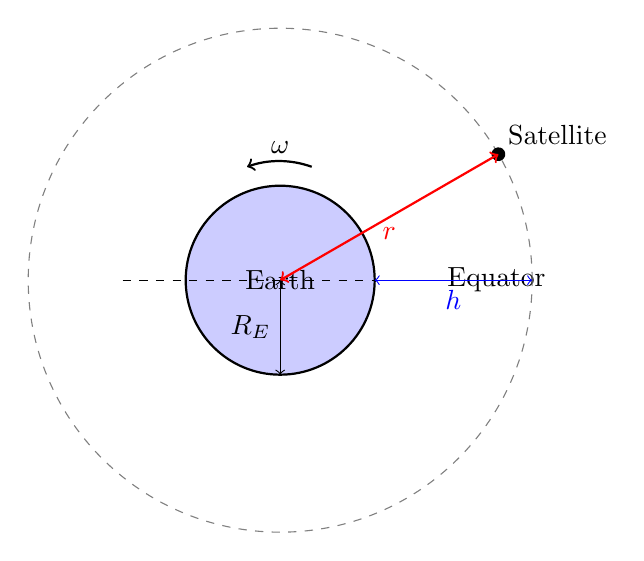
\begin{tikzpicture}[scale=0.8]
    % Earth
    \draw[thick, fill=blue!20] (0,0) circle (1.5);
    \node at (0,0) {Earth};
    \draw[dashed] (-2.5,0) -- (2.5,0) node[right] {Equator};
    
    % Orbit
    \draw[dashed, color=gray] (0,0) circle (4);
    
    % Satellite
    \begin{scope}[rotate=30]
        \draw[fill=black] (4,0) circle (0.1) node[above right] {Satellite};
        \draw[<->, thick, red] (0,0) -- (4,0) node[midway, below] {$r$};
    \end{scope}
    
    % Radius and Altitude labels
    \draw[<->] (0,-1.5) -- (0,0) node[midway, left] {$R_E$};
    \draw[<->, blue] (1.5,0) -- (4,0) node[midway, below] {$h$};
    
    % Rotation
    \draw[->, thick] (0.5,1.8) arc (70:110:1.5);
    \node at (0,2.1) {$\omega$};
\end{tikzpicture}
\end{center}

The geostationary orbit radius is approximately \textbf{42,164 km} from the Earth's center, which corresponds to an altitude of roughly \textbf{35,793 km} above the surface.


% -------------------------------------------------------------------------------------------------

\item \textit{The coefficient of static friction is $\mu_{0}$. At what angle $\alpha$ will the object begin to slide?}

\medskip

Determine the angle $\alpha$ at which an object placed on an inclined plane begins to slide, given the coefficient of static friction $\mu_0$.

Consider an object of mass $m$ on a plane inclined at an angle $\alpha$. The forces acting on the object are:
\begin{itemize}
    \item Gravity ($mg$), which has components:
    \begin{itemize}
        \item Parallel to the plane: $F_{\parallel} = mg \sin\alpha$
        \item Perpendicular to the plane: $F_{\perp} = mg \cos\alpha$
    \end{itemize}
    \item The normal force: $N = mg \cos\alpha$
    \item The force of static friction: $f_s \leq \mu_0 N$
\end{itemize}

The object starts to move when the component of gravity pulling it down the slope equals the maximum possible static friction:
\begin{equation}
    mg \sin\alpha = \mu_0 \cdot mg \cos\alpha
\end{equation}

Dividing both sides by $mg \cos\alpha$ (assuming $\alpha < 90^\circ$):
\begin{equation}
    \frac{\sin\alpha}{\cos\alpha} = \mu_0 \implies \tan\alpha = \mu_0
\end{equation}

Thus, the critical angle is:
\begin{equation}
    \alpha = \arctan(\mu_0)
\end{equation}

The following figure illustrates the forces acting on the object:

\begin{center}
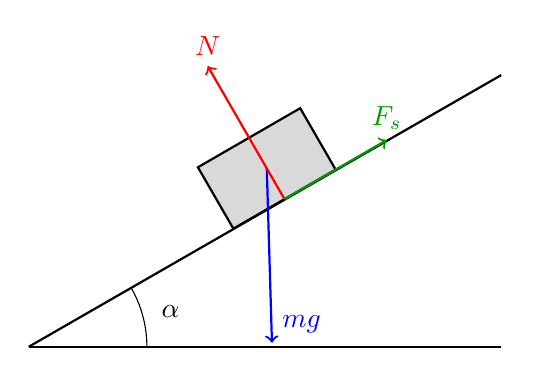
\begin{tikzpicture}[scale=1.5]
    % Inclined plane
    \draw[thick] (0,0) -- (4,0) node[right] {};
    \draw[thick] (0,0) -- (4,2.3) node[right] {};
    \draw (1,0) arc (0:30:1);
    \node at (1.2,0.3) {$\alpha$};

    % Box
    \begin{scope}[rotate=30]
        \draw[fill=gray!30, thick] (2,0) rectangle (3,0.6);
        \coordinate (C) at (2.5,0.3); % Center of mass
        
        % Force arrows
        \draw[->, blue, thick] (2.5,0.3) -- (1.8,-1.0) node[above right] {$mg$}; % Gravity
        \draw[->, red, thick] (2.5,0) -- (2.5,1.3) node[above] {$N$}; % Normal
        \draw[->, green!60!black, thick] (2.5,0) -- (3.5,0) node[above] {$F_s$}; % Friction
    \end{scope}
\end{tikzpicture}
\end{center}

An object will begin to slide when the tangent of the inclination angle reaches the coefficient of static friction.

% -------------------------------------------------------------------------------------------------

\pagebreak
\item \textit{A $2\,\text{kg}$ object slides down from the top of a $3\text{-meter-high}$ inclined plane that makes an angle of $30^\circ$ with the horizontal. What is the velocity of the object when it reaches the bottom of the incline, starting from rest at the top, if:
\begin{enumerate}
    \item[(a)] there is no friction between the object and the incline?
    \item[(b)] the coefficient of friction is $0.05$?
\end{enumerate}}

\medskip

Here,
\begin{itemize}
    \item Height: $h = 3\,\text{m}$
    \item Angle: $\alpha = 30^\circ$
    \item Length of the slope: $L = \frac{h}{\sin\alpha} = \frac{3}{\sin(30^\circ)} = 6\,\text{m}$
    \item Mass: $m = 2\,\text{kg}$
    \item Gravity: $g \approx 9.81\,\text{m/s}^2$
\end{itemize}

\begin{center}
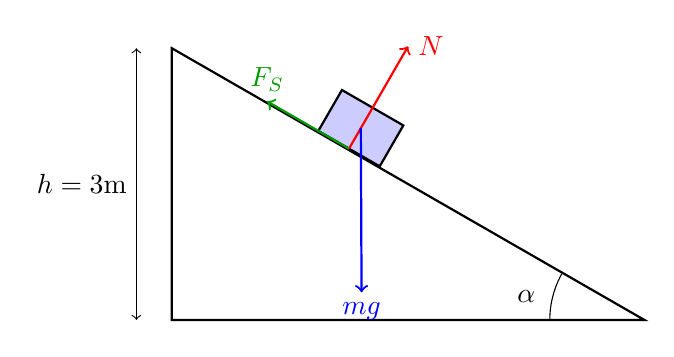
\begin{tikzpicture}[scale=1.5]
    % Slope
    \draw[thick] (0,0) -- (4,0) -- (0,2.3) -- cycle;
    \draw (3.2,0) arc (180:150:0.8);
    \node at (3,0.2) {$\alpha$};
    
    % Object
    \begin{scope}[shift={(1.5,1.45)}, rotate=-30]
        \draw[fill=blue!20, thick] (-0.3,0) rectangle (0.3,0.4);
        \coordinate (G) at (0,0.2);
        % Forces
        \draw[->, red, thick] (0,0) -- (0,1) node[right] {$N$};
        \draw[->, green!60!black, thick] (0,0) -- (-0.8,0.0) node[above] {$F_S$};
        \draw[->, blue, thick] (G) -- (0.7,-1) node[below] {$mg$};
    \end{scope}
    \draw[<->] (-0.3,0) -- (-0.3,2.3) node[midway, left] {$h=3$m};
\end{tikzpicture}
\end{center}

\begin{enumerate}
\item[(a)] Case without friction. Using the principle of conservation of energy:
\begin{equation}
    mgh = \frac{1}{2}mv^2 \implies v = \sqrt{2gh}
\end{equation}
Substituting the values:
\begin{equation*}
    v = \sqrt{2 \cdot 9.81 \cdot 3} = \sqrt{58.86} \approx 7.67\,\text{m/s}
\end{equation*}

\item[(b)] Case with friction ($\mu = 0.05$)
The work-energy theorem states: $mgh - W_{friction} = \frac{1}{2}mv^2$.
The friction force is $f_k = \mu N = \mu mg \cos\alpha$.
The work done by friction is $W_f = f_k \cdot L$.
\begin{eqnarray*}
    mgh - \mu mg \cos\alpha \cdot \frac{h}{\sin\alpha} &=& \frac{1}{2}mv^2 \\
    gh(1 - \mu \cot\alpha) &=& \frac{1}{2}v^2 \\
    v &=& \sqrt{2gh(1 - \mu \cot\alpha)}
\end{eqnarray*}
Substituting the values ($\cot 30^\circ = \sqrt{3}$):
\begin{equation*}
    v = \sqrt{2 \cdot 9.81 \cdot 3 \cdot (1 - 0.05 \cdot 1.732)} \approx \sqrt{58.86 \cdot 0.9134} \approx 7.33\,\text{m/s}
\end{equation*}
\end{enumerate}

Therefore, 
\begin{itemize}
    \item[(a)] Velocity without friction: \textbf{7.67 m/s}
    \item[(b)] Velocity with friction: \textbf{7.33 m/s}
\end{itemize}

% -------------------------------------------------------------------------------------------------

\pagebreak
\item \textit{A string is wound around a solid cylinder with radius $R = 0.5\,\text{m}$ and mass $M = 26\,\text{kg}$. Two objects with a combined mass of $12\,\text{kg}$ are hanging from the ends of the string. Upon release, the cylinder accelerates with an angular acceleration of $\beta = 3.2\,\text{rad/s}^2$. The string does not slip.
\begin{itemize}
    \item[(a)] Find the individual masses ($m_1, m_2$) of the two objects.
    \item[(b)] Calculate the total kinetic energy of the system at $t = 3\,\text{s}$.
\end{itemize}}

\medskip

Let $m_1$ be the larger mass. The linear acceleration is $a = \beta R = 3.2 \cdot 0.5 = 1.6\,\text{m/s}^2$. 
The equations of motion are:
\begin{eqnarray}
    m_1 g - T_1 &=& m_1 a \\
    T_2 - m_2 g &=& m_2 a \\
    (T_1 - T_2)R &=& I\beta = \frac{1}{2}MR^2\beta = \frac{1}{2}MaR
\end{eqnarray}
Combining these yields:
\begin{equation}
    (m_1 - m_2)g - (m_1 + m_2)a = \frac{1}{2}Ma
\end{equation}
Substituting the known values ($g=9.81$):
\begin{equation*}
    (m_1 - m_2)9.81 - 12(1.6) = 0.5(26)(1.6) \implies m_1 - m_2 \approx 4.077\,\text{kg}
\end{equation*}
Solving the system with $m_1 + m_2 = 12$:
\begin{equation*}
    m_1 \approx 8.04\,\text{kg}, \quad m_2 \approx 3.96\,\text{kg}
\end{equation*}

At $t = 3\,\text{s}$, the velocity is $v = at = 1.6 \cdot 3 = 4.8\,\text{m/s}$, and $\omega = v/R = 9.6\,\text{rad/s}$.
The total kinetic energy is the sum of translational and rotational energies:
\begin{equation}
    E_{total} = \frac{1}{2}(m_1 + m_2)v^2 + \frac{1}{2}I\omega^2 = \frac{1}{2}(m_1 + m_2)v^2 + \frac{1}{2}(\frac{1}{2}MR^2)\omega^2
\end{equation}
\begin{equation*}
    E_{total} = \frac{1}{2}(12)(4.8)^2 + \frac{1}{4}(26)(0.5^2)(9.6^2) = 138.24 + 74.5 \approx 212.74\,\text{J}
\end{equation*}

\begin{center}
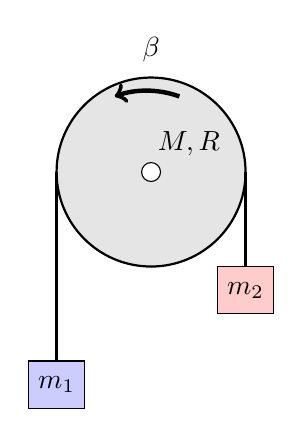
\begin{tikzpicture}[scale=1.2]
    % Cylinder
    \draw[thick, fill=gray!20] (0,0) circle (1);
    \draw[fill=white] (0,0) circle (0.1);
    \node at (0.4,0.3) {$M, R$};
    
    % Strings
    \draw[thick] (-1,0) -- (-1,-2);
    \draw[thick] (1,0) -- (1,-1);
    
    % Masses
    \draw[fill=blue!20] (-1.3,-2) rectangle (-0.7,-2.5) node[midway] {$m_1$};
    \draw[fill=red!20] (0.7,-1) rectangle (1.3,-1.5) node[midway] {$m_2$};
    
    % Forces
    \draw[->, ultra thick] (0.3,0.8) arc (70:110:1);
    \node at (0,1.3) {$\beta$};
\end{tikzpicture}
\end{center}

% -------------------------------------------------------------------------------------------------

\item \textit{Estimate the average depth of the Pacific Ocean if a tsunami takes 6 hours to travel from Hawaii to Alaska. (Note: The propagation speed of shallow-water waves is $v=\sqrt{gh}$.)}


So,
\begin{itemize}
    \item Distance: $d = 4 \times 10^6\,\text{m}$
    \item Time: $t = 6 \times 3,600 = 21,600\,\text{s}$
    \item Gravity: $g = 9.81\,\text{m/s}^2$
\end{itemize}

The average velocity of the tsunami is:
\begin{equation}
    v = \frac{d}{t} = \frac{4,000,000}{21,600} \approx 185.19\,\text{m/s}
\end{equation}

Using the shallow-water wave formula $v^2 = gh$:
\begin{equation}
    h = \frac{v^2}{g} = \frac{(185.19)^2}{9.81} \approx \frac{34295.3}{9.81} \approx 3,495.9\,\text{m}
\end{equation}

\begin{center}
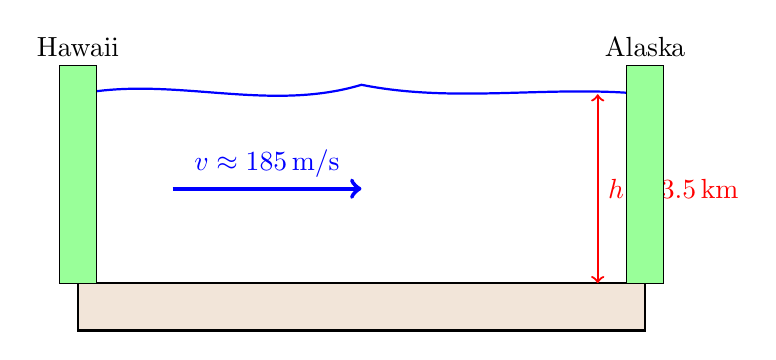
\begin{tikzpicture}[scale=1.2]
    % Ocean surface
    \draw[blue, thick] (0,2) .. controls (1,2.2) and (2,1.8) .. (3,2.1) .. controls (4,1.9) and (5,2.1) .. (6,2);
    
    % Ocean floor
    \draw[thick, fill=brown!20] (0,0) -- (6,0) -- (6,-0.5) -- (0,-0.5) -- cycle;
    
    % Depth indicator
    \draw[<->, thick, red] (5.5,0) -- (5.5,2) node[midway, right] {$h \approx 3.5\,\text{km}$};

    % Landmarks
    \draw[fill=green!40] (-0.2,0) rectangle (0.2,2.3);
    \node[above] at (0,2.3) {Hawaii};
    \draw[fill=green!40] (5.8,0) rectangle (6.2,2.3);
    \node[above] at (6,2.3) {Alaska};

    % Velocity arrow
    \draw[->, ultra thick, blue] (1,1) -- (3,1) node[midway, above] {$v \approx 185\,\text{m/s}$};
\end{tikzpicture}
\end{center}

Therefore, with a travel time of 6 hours over a 4,000 km distance, the estimated average depth of the ocean is approximately \textbf{3,496 meters}. This result is very close to the actual average depth of the Pacific Ocean.

\end{enumerate}

\end{document}


\bigskip

\rightline{Dr.~Gabor~FACSKO}
\rightline{\textit{facsko.gabor@uni-obuda.hu}}

\vfill

\end{document}
